\documentclass[a4paper,11pt,onecolumn]{article}
\usepackage[hscale=0.8,vscale=0.9]{geometry}
\usepackage[parfill]{parskip}
\usepackage{amsmath}
\usepackage{amsfonts}
\usepackage{graphicx}
\usepackage{subfigure}
\usepackage{wrapfig}
\usepackage{amssymb}

\newcommand{\eat}[1]{}

\begin{document}
\include{weld-defns}
\title{Research Statement}
\author{Niranjan Balasubramanian}
\maketitle

My research spans two broad areas: Information retrieval and information extraction. I am motivated by applications that require computer systems to extract, organize, understand and reason with information in natural language texts. Pursuit of this long-standing Artificial Intelligence vision has tremendous societal and scientific impacts. Applications such as Question answering systems, event extraction and summarization systems go far beyond web search in terms of providing easy access and organization to the vast amounts information on the web. These are challenging applications that require large scale open-domain knowledge. 

Consider a system answering a 4th grade science question:  ``Which is the best conductor of electricity? (A) metal fork (B) rubber boat''. To answer this question a system can use the knowledge that i) a metal fork is made of metal, ii) metals conduct electricity, and iii) properties of a metal apply to things made of metal and reason with these facts to arrive at the answer. Consider an event extraction system that is "reading" an article about an arrest event. If the system had knowledge about what a typical arrest event is -- i.e., who the key actors are and what their roles are -- then it can use that information to identify the salient pieces to extract from the article. 

My current research focuses on developing methods for extracting such large scale open-domain knowledge and robust mechanisms for applying this knowledge. To be widely applicable, methods for constructing such semantic knowledge must meet the following design goals. They must scale to arbitrary domains, model semantics without ambiguity, and generalize to unseen contexts. I use Open Information Extraction (Open IE) techniques to extract open-domain relations and representations augmented with semantic classes to reduce ambiguity and improve generalization.

My research methods are centered on identifying the core aspects of the problem space through careful analysis of existing systems and data. For instance, in my work on mobile web search, I conducted a systematic study of data transfer costs in cellular networks and identified a key inefficiency. In addition to improving web search efficiency, this insight led to a large body of research aimed at minimizing this inefficiency for a wide variety of mobile applications.~\footnote{Has more than 350 citations.} As part of my thesis work, I analyzed performance of different types of query models and ranking functions and proposed a novel method for combining them on a per-query basis. In my work on event schemas, I analyzed output from previous system to identify the key shortcomings of underspecified representations used in prior work. The insights led to a better representation that vastly improved the quality of the schemas. 

Here I describe some of my research and lay out my vision for future work.

\eat{My vision is to develop methods for extracting large scale open-domain knowledge. My research is motivated by applications such as event extraction and question answering, which require computer systems to extract, understand and reason with information present in natural language text. For example, event extraction systems use knowledge about events to guide extraction.}

\eat{
They use event schemas (also known as templates) to identify which pieces of information to extract about an event. For example, an arrest schema will contain the arresting agent, the person who gets arrested, and the judge who rules on the case. One of my main research focus is to automatically build such event models (also known as event schemas) from text without any human effort.

To be widely applicable, methods for constructing such semantic knowledge must meet the following design goals. They must scale to arbitrary domains, model semantics without ambiguity, and generalize to unseen contexts.
}
\eat{First, they must scale to arbitrary domains and hence should not rely on domain specific models or resources. Second, the representation should be specific enough to model the semantics without ambiguity. Underspecified representations allow for robust estimation but often at the expense of increased ambiguity. For instance, when modeling events, a verb only representation will conflate relations that differ by the semantics of an attached proposition (e.g, in a lawsuit scenario the object of ``file by'' is a plaintiff and ``file against'' is a defendant).\eat{Further, using a verb only representation (without prepositions) might provide robust models for more verbs but cover fewer relations.} Finally, the methods must allow for generalization to new unseen contexts. For example, a semantic model about a smart-phone must generalize to be applicable for a related but newer context of Google glass.
}
\eat{The goal of my work is to build methods that yield open domain, broad coverage semantic knowledge through careful representations that can be easily extracted using open domain technologies. My past work focused on building two types of semantic knowledge a) Rel-grams -- A form of entailment knowledge that captures what relation is likely to follow a given relation, and b) Open Schemas -- A model of the key actors and the roles they play in a scenario. }

{\bf NLP [EMNLP 2013, AKBC-WEKEX 2012, 2013]}

{\em Modeling Events}

Event schemas that specify actors and their roles within events are widely used in event extraction. Figure~\ref{fig:arrest} shows an example arrest schema. The key actors are an arresting agent who arrests and charges a suspect, a lawyer who represents the suspect and a judge who rules on the case. Until recently, these were hand-engineered and consequently were limited to a small number of domains. My research aims to automatically generate these schemas from text with no manual effort with a specific focus on generating coherent schemas.

The main premise behind my work is that an accurate model of co-occurring actors and their actions can provide a basis for automatically generating schemas. The main challenge is in defining a suitable representation for the actions. My analysis of the output from a previous system showed that simpler (subject, verb) and (verb, object) pairs are underspecified representations that split critical context. In response, I developed an Open IE triple-based solution that uses a (Arg1, Relation, Arg2) triple that captures more specific information about the actions and reduces ambiguity. However, this reduction in ambiguity comes at a cost of increased sparsity and reduced generalization. 
\begin{wrapfigure}{r}{0.4\textwidth}
	\vspace{-2ex}
	\begin{center}
	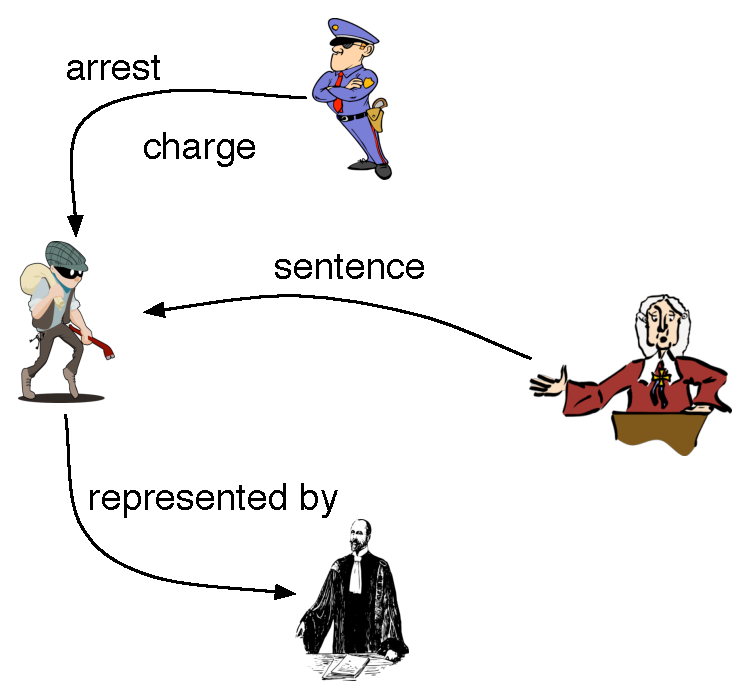
\includegraphics[width=2.5in,height=2in]{figures/arrest-scenario} 	
	\vspace{-2ex}
	\caption{\label{fig:arrest} {\small Arrest schema: A model for an arrest scenario including key actors, the police, the suspect, judge etc. and their roles.}}
	\vspace{-2ex}
	\end{center}
\end{wrapfigure}
To counter this issue, I represent arguments using semantic classes, which allows the model to generalize beyond the specific entities to new unseen contexts. The relational co-occurrence model (Rel-grams) built over this triple representation yields a form of entailment type knowledge~\cite{balasubramanian-akbc12} and produces schemas that are more coherent than state-of-the-art systems~\cite{balasubramanian-emnlp13}.

{\bf Question Answering}

Achieving human-level performance on tasks that require intelligence has a long tradition in the history of Artificial Intelligence~\cite{}. As one of the foundational members of the Allen Institute for Artificial Intelligence, I am co-leading efforts to design and develop a QA system that is capable of passing a 4th grade science exam. This is an exciting long-term research that seeks to address several fundamental challenges in representation, extraction and reasoning all in the context of a single task.

As a first step in this task, we studied the knowledge requirements for passing a 4th grade science exam~\cite{clark-akbc13}. The knowledge requirements summarized in Figure~\ref{fig:akbc} shows that this is a challenging task requiring a wide range of knowledge and robust reasoning methods. In addition to factual knowledge (e.g., iron conducts electricity), we identify three other types of useful knowledge: 1) Definitional knowledge, 2) Domain knowledge expressed via general purpose relations such as cause/effect, entity/function, 3) Implications representing domain and background knowledge (e.g., animal breathes oxygen $-$enables$\rightarrow$ animal make energy), and 4) Qualitative domain models (e.g., Reasoning with predator-prey models: If population of snakes rise, what happens to the population of frogs?).

\begin{wrapfigure}{l}{0.4\textwidth}
	\vspace{-2ex}
	\begin{center}
	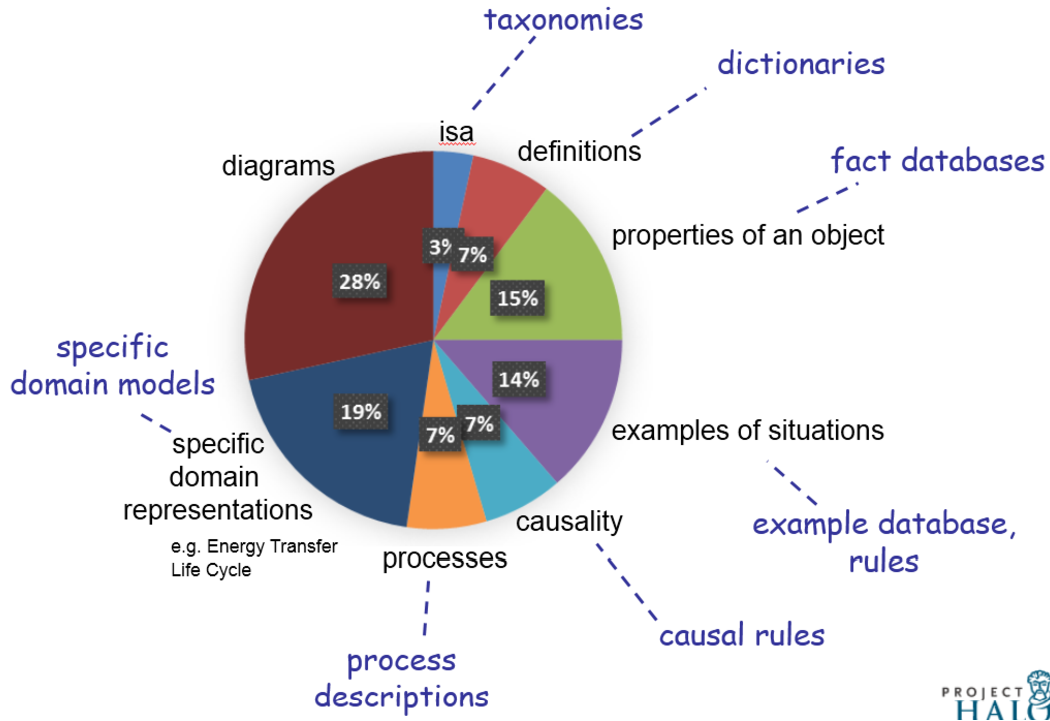
\includegraphics[width=3in,height=2in]{figures/akbc} 	
	\vspace{-2ex}
	\caption{\label{fig:akbc} {\small Knowledge Requirements for passing a 4th Grade Science Exam}}
	\vspace{-2ex}
	\end{center}
\end{wrapfigure}

We are building a wide array of solutions to address these difficult challenges. We extract definitional and general purpose relations such as cause/effect and entity/function using hand-generated lexico-syntactic patterns that exploit strong regularities in language. We use Open IE style relations to represent information but expand them to cover nested relations. In addition, we also use facts extracted using a state-of-the-art Open IE extractor.

I am building a probabilistic reasoning framework that uses these knowledge sources to answer questions. Specifically, I cast question answering as a marginal inference problem in a Markov Logic Network (MLN) with implication knowledge as first-order rules and nested relations as evidence. Different from traditional applications of MLNs, the knowledge and rules here are textual, as a result of which several gaps arise due to vocabulary mismatch. To address these lexical gaps, I created an iterative bi-directional search algorithm that uses coarse but fast methods to locate plausible gaps and bridges them using deeper textual entailment techniques. One of the key challenges here is to restrict the backward-search to a feasible space. 

\eat{For acquiring definitional knowledge we exploit the strong regularities in definitional language to produce open ie style relations representing the definition. A typical definition includes the class or semantic type information about the term and one or more {\em definitional} properties. We used a handful of patterns covered 50\% of the definitions mined from the web at a high precision. For extracting domain knowledge, we use hand-generated dependency patterns to extract general purpose relations such as cause/effect. I am cure
}

{\bf Information Retrieval [SIGIR 2010, CIKM 2009, IMC 2009, CoNext 2012]}


{\bf Combining Alternatives}

The IR research community continuously develops query representations, retrieval models, and various ranking algorithms. As part of my thesis, I developed a dynamic query-dependent approach for combining different alternatives. The main premise behind my thesis is that different alternatives work well for different queries. For example, a navigation query (intent to visit a specific url) is well served by user click based features, whereas a informational query is better served by query-document match features. If we can select the best choice(s) for a given query, then we can further improve retrieval performance. 

To this end, I developed a novel method that estimates the relative performance of the alternatives with respect to a baseline using easy to compute retrieval features~\cite{balasubramanian-sigir10a}. The key insight behind this method was that accurate estimation of the absolute effectiveness value was not essential. The estimation only needed to induce a good ordering of the available alternatives. This relative estimation method outperformed using the single best alternative for query representations~\cite{balasubramanian-sigir10b} and ranking functions~\cite{balasubramanian-sigir10c}. 


{\bf Topic Pages}

As an alternative to the typical web search paradigm, I built a system that automatically generates wikipedia like pages for topics~\cite{balasubramanian-icsc2010}. The primary challenge here is to identify the salient aspects pertaining to the topic. I exploited web search logs which aggregate user interests about topics to build diverse aspect models on topics.To generalize to topics beyond those that are observed in the search logs, we generalized the aspect models to include information about related entities. A second challenge here is to extract and organize information pertaining to the diverse aspects in a coherent fashion. I built a sentence extractor that identifies most typical connection between the topic and its aspect and used simple word-precedence models to organize the retrieved sentences. The resulting topic pages outperformed state-of-the-art summarization systems in terms of grammaticality, salience and coherence.

{\bf Mobile Search}

I studied the impact of system constraints on web search from mobile phones. I conducted a systematic study of how network activity consumed energy in mobile phones. My study revealed that energy consumption also depended on inter-transfer times in addition to the size of the data being transferred~\cite{balasubramanian-imc09}. Based on this insight, I designed interaction strategies that reduced the energy consumption of web search applications. The key finding in this work spawned a large body of research aimed at minimizing the energy inefficiency. 

I also worked on {\em FindAll}, a mobile search engine aimed at improving local availability of previously visited documents. Because indexing on the phone is expensive, the system must balance local availability against resource usage and energy consumption. Using actual search logs from mobile users, we learned user-specific re-finding patterns to predict when a user is likely to re-find documents. Using this predictive model, FindAll selectively indexes documents when cost of indexing is lower than cost of re-finding the document over the network. Evaluations show that FindAll dramatically improves local availability for heavy users without increasing the energy costs.

{\bf Future Work}

I am interested in extracting open-domain knowledge from text. In particular I want to extracting script-like descriptions of open-domain events and processes. My past work on Rel-grams and open event schemas provides a starting point but much work remains do be done. I am also interested in methods that can handle the gaps and noise inherent in such automatically extracted knowledge.
% In particular I wish to exploit existing semantic resources and extraction capabilities to build richer semantic structures at scale. I am also interested in developing robust application mechanisms to handle the gaps and noise inherent in such automatically extracted knowledge.

{\bf Script-like Knowledge}

Scripts are general purpose descriptions of events or scenarios. They include the key actors, their actions, and causal and temporal relationship between the different actions~\cite{schank-scripts75}. A dinner script for example includes an ordered sequence of actions: An actor going to a restaurant, placing an order with a waiter, eating the food, and then paying the bill. These scripts provide valuable general purpose knowledge but aggregating high-quality scripts is a challenging task because many aspects of this knowledge are often implicit making it harder to detect. I am interested in methods that can aggregate and generalize from explicitly mentioned aspects. %These are challenging problems. I am interested in developing bootstrapping solutions that use high-precision methods to detect these connections where possible and then aggregate over generalizations to infer connections in new documents. 

Scripts can fill in missing connections in texts. If we read the sentences ``John went to Bill's restaurant and ordered steak. He paid \$50 for the meal.'', we easily infer that John most likely ate the steak. Identifying such causal links is challenging. Causal links can be explicit (e.g., John ate lunch early {\em because} he was hungry) or implicit (e.g., John ate lunch early. He was hungry). The explicit mentions can be identified more reliably using lexical cues such as the causal connective {\em because}. There are other structural constraints such as transitivity (i.e., A causes B and B causes C $\rightarrow$ A causes C) which can further improve precision. The bootstrapping task here is to detect explicit links with high-precision and then learn patterns over generalized representations of the actors and their actions. 

%A bootstrapping model can first detect the explicit links with high precision and then aggregate these causal links over generalized representations of the actors and the actions. For example, we can learn that if X ate then it was most likely because X was hungry.

Scripts can help resolve ambiguous references in texts. Consider the following sentence: ``[People] travel to see their [families] when [they] find cheap flights to take [them]". [they] can resolve to families or [people]. Resolving pronouns in this sentence requires the system to know that the entity that travels is the one that is likely to find flights. Rel-grams provides a framework for aggregating this kind of background knowledge. One of the key challenges is the precision/recall trade-off. Past attempts at improving co-reference by adding semantics have mixed results because they either lack coverage or are too imprecise due to over-generalization. Rel-grams addresses this to some extent by including more context to improve accuracy and semantic classes to improve generalization. 

Script-like knowledge provides a powerful model for extracting information about events. Scripts provide a template for extracting salient information about events by specifying the key actors and their actions.My past work on open event schemas produced coherent models of events in terms of the key actors and their roles and thus provide a strong basis constructing high-quality event extractors at scale. Expanding schemas to include extractors can also be viewed as a bootstrapping procedure starting from a strong high-quality model of an event. As with any bootstrapping approach the challenges are in finding appropriate sources for expansion and avoiding drifting from the source model. 


\eat{They are a powerful model of events including key actors, their roles and causal relationships~\cite{schank-scripts75}. Event schemas provide a start for building these script-like knowledge about events. However, they have limited generalization due to the use of a relatively smaller set of semantic classes. For example, the schemas cannot distinguish between a sports person and a baseball player. Moreover, the schemas do not include causality relations or temporal ordering of the actions within the schema. For example, the arrest schema does not  include information about whether the arrest precedes filing charges or vice versa. First, I wish to exploit high-quality entity linking systems and semantic resources such as NELL to expand to a much larger hierarchy of semantic classes. This raises interesting challenges: It is difficult to decide what semantic class to assign to a specific relation. In some cases a general category is preferable (e.g., ([sportsperson], failed, [drug test]) ), whereas in others a more specific category is preferable (e.g., ([baseball player], scored, home run)).  Second, I wish to leverage causality detection methods to annotate the schemas with causal relations. Even though these methods are not perfect, we can devise techniques that can prune errors in aggregation. }

\eat{Script like knowledge provide powerful models of events at discourse level by including key actors, their roles and causal relationships~\cite{schank-scripts75}. Rel-grams and schemas provide a start. However, their generalization is somewhat limited due to use of a limited set of semantic classes chosen in an ad-hoc fashion. Further, they do not include other valuable discourse relations such as causality and temporal ordering. First, I wish to exploit high-quality entity linking systems and semantic resources such as NELL to expand to a much larger hierarchy of semantic classes. This raises interesting challenges. For example, it is difficult to decide what semantic class to assign to a specific relation. In some cases a general category is preferable (e.g., ([sportsperson], failed, [drug test]) ), whereas in others a more specific category is preferable (e.g., ([baseball player], scored, home run)).  Second, I wish to leverage causality detection methods to annotate the schemas with causal relations. Even though these methods are not perfect, we can devise techniques that can prune errors in aggregation. }

\eat{
{\bf Event Extraction and Reference Resolution}

Scalable event extraction requires open domain models of events. Existing methods have used manual templates or use probabilistic methods that are unlikely to scale.%Past attempts have either used manual templates~\cite{patwardhan-emnlp09} or have used probabilistic methods that limit application to large scale open domain data~\cite{cheung-naacl13,chambers-emnlp13}. 
Open event schemas are coherent models of the key actors and their roles and thus provide a strong basis constructing high-quality extractors at scale. Expanding schemas to include extractors can be viewed as a bootstrapping procedure starting from a strong high-quality model of an event. As with any bootstrapping approach the challenges are in finding appropriate sources for expansion and avoiding drifting from the source model. 

Resolving co-reference is a challenging problem that requires broad semantic knowledge in the form of type constraints. Consider the following sentence: ``[People] travel to see their [families] when [they] find cheap flights to take [them]". [they] can resolve to families or [people]. Resolving pronouns in this sentence requires the system to know that the entity that travels is the one that is likely to find flights. Rel-grams provides a framework for aggregating this kind of background knowledge. One of the key challenges is the precision/recall trade-off. Past attempts at improving co-reference by adding semantics have mixed results because they either lack coverage or are too imprecise due to over-generalization. Rel-grams addresses this to some extent by including more context to improve accuracy and semantic classes to improve generalization.

{\bf Process Knowledge}
}
{\bf Extracting Implications}

Passing grade science exams requires extraction and reasoning with implications knowledge. A large portion of knowledge in textbooks and study guides require complex nested structures for representation. In addition to increasing the complexity of extraction, this also makes the inference problem harder. I intend to explore hybrid architectures which allow for reasoning with representations with varying degrees of complexity to avoid inference with complex structures where possible. 

Reasoning with knowledge extractedd from texts requires robust approaches. However, past attempts at producing robust approaches has mainly resulted in everything in the kitchen sink style approaches. This has led to measured progress in textual entailment tasks, but they haven't shed much insights into the properties of the systems themselves or on the problem space. In contrast, I am interested in approaches that preserve the deductive style of inference as much as possible while falling back to distributional methods to bridge gaps but within the inference framework. This I believe combines the best of both worlds -- retains the robustness of the entailment style methods while also explicitly showing where the current knowledge is lacking or where textual reasoning is required. The question answering project is a great testbed to test these ideas.

{\bf Information Retrieval}

Lastly, I am interested in exploiting semantic knowledge for Information retrieval. In the past, IR applications have had mixed success with using semantic resources. The key limiting factor was the coverage of the resources used and scalability of the methods. Recent advances in large scale language processing and knowledge extraction techniques provide an ideal opportunity to test integration of semantics. Open Information Extraction presents an ideal starting point. It provides fast and a shallow representation of salient information in a corpus that can be used to improve retrieval. 


\eat{
%Resolving co-reference is a challenging problem that requires broad semantic knowledge~\cite{}. Consider the following sentence: ``[People] travel to see their [families] when [they] find cheap flights to take [them]". [they] can resolve to families or [people]. Resolving pronouns in this sentence requires the system to know that the entity that travels is the one that is likely to find flights. Rel-grams provides a framework for aggregating this kind of background knowledge. One of the key challenges is the precision/recall trade-off. Past attempts at improving co-reference by adding semantics have mixed results because they either lack coverage or are too imprecise due to over-generalization. Rel-grams addresses this to some extent by including more context to improve accuracy and semantic classes to improve generalization. [But more needs to be done... What?]

Question answering for passing grade science exams requires extraction and reasoning with implications knowledge. The work on Rel-grams provides a starting point but is seriously limited especially in terms of the amount of context captured. For example, consider the question about 
...\\
...\\
...\\


Reasoning with semantic resources constructed from texts requires robust approaches. However, past attempts at producing robust approaches has mainly resulted in everything in the kitchen sink style approaches. This has led to measured progress in textual entailment tasks, but they haven't shed much insights into the properties of the systems themselves or on the problem space. In contrast, I am interested in approaches that preserve the deductive style of inference as much as possible while falling back to distributional methods to bridge gaps but within the inference framework. This I believe combines the best of both worlds -- retains the robustness of the entailment style methods while also explicitly showing where the current knowledge is lacking or where textual reasoning is required. The question answering project is a great testbed to test these ideas...\\

Lastly, I am interested in exploiting semantic resources for Information retrieval. In the past, IR applications have had mixed success with using semantic resources. The key limiting factor was the coverage of the resources used...\\
}
{\small
\bibliographystyle{plain}
\bibliography{../research-statement,../kia}
}
\end{document}


\eat{As a first step in this challenging task, we studied the knowledge requirements for passing this exam~\cite{clark-akbc13}. The analysis presented several critical insights into the challenges that lay ahead. Figure~\ref{fig:knowledge-wheel} shows the required knowledge categories as a wheel. In addition to factual knowledge (e.g., iron conducts electricity), we identify three other types of useful knowledge: 1) Definitional knowledge: Terminology questions often test the ability of students to match terminology to its description. 2) Domain knowledge: A wide variety of domain knowledge expressed via general purpose relations such as cause/effect, action/purpose, entity/function and object/property. 3) Implications: To answer many questions the system requires knowledge represented as implications (e.g, animal breathes oxygen $-$enables$\rightarrow$ animal make energy). 4) Domain models: Modeling questions involve ability to reason with certain types of models (e.g. Reasoning with predator-prey models: If population of snakes rise, what happens to the population of frogs?). }
